\documentclass[leqno, openany]{memoir}
\setulmarginsandblock{3.5cm}{3.5cm}{*}
\setlrmarginsandblock{3cm}{3.5cm}{*}
\checkandfixthelayout

\usepackage{amsmath}
\usepackage{amssymb}
\usepackage{amsthm}
%\usepackage{MnSymbol}
\usepackage{bm}
\usepackage{accents}
\usepackage{mathtools}
\usepackage{tikz}
\usetikzlibrary{calc}
\usetikzlibrary{automata,positioning}
\usepackage{tikz-cd}
\usepackage{forest}
\usepackage{braket} 
\usepackage{listings}
\usepackage{mdframed}
\usepackage{verbatim}
\usepackage{physics}
\usepackage{caption}
\usepackage{subcaption}
%\usepackage{/home/patrickl/homework/macaulay2}

%font
\usepackage[osf]{mathpazo}
\usepackage{microtype}

%CS packages
\usepackage{algorithmicx}
\usepackage{algpseudocode}
\usepackage{algorithm}

% typeset and bib
\usepackage[english]{babel} 
\usepackage[utf8]{inputenc} 
\usepackage[backend=biber, style=alphabetic]{biblatex}
\usepackage[bookmarks, colorlinks, breaklinks]{hyperref} 
\hypersetup{linkcolor=black,citecolor=black,filecolor=black,urlcolor=black}

% other formatting packages
\usepackage{float}
\usepackage{booktabs}
\usepackage{enumitem}
\usepackage{csquotes}
\usepackage{titlesec}
\usepackage{titling}
\usepackage{fancyhdr}
\usepackage{lastpage}
\usepackage{parskip}

\usepackage{lipsum}

% delimiters
\DeclarePairedDelimiter{\gen}{\langle}{\rangle}
\DeclarePairedDelimiter{\floor}{\lfloor}{\rfloor}
\DeclarePairedDelimiter{\ceil}{\lceil}{\rceil}


\newtheorem{thm}{Theorem}[section]
\newtheorem{cor}[thm]{Corollary}
\newtheorem{prop}[thm]{Proposition}
\newtheorem{lem}[thm]{Lemma}
\newtheorem{conj}[thm]{Conjecture}
\newtheorem{quest}[thm]{Question}

\theoremstyle{definition}
\newtheorem{defn}[thm]{Definition}
\newtheorem{defns}[thm]{Definitions}
\newtheorem{con}[thm]{Construction}
\newtheorem{exm}[thm]{Example}
\newtheorem{exms}[thm]{Examples}
\newtheorem{notn}[thm]{Notation}
\newtheorem{notns}[thm]{Notations}
\newtheorem{addm}[thm]{Addendum}
\newtheorem{exer}[thm]{Exercise}

\theoremstyle{remark}
\newtheorem{rmk}[thm]{Remark}
\newtheorem{rmks}[thm]{Remarks}
\newtheorem{warn}[thm]{Warning}
\newtheorem{sch}[thm]{Scholium}


% unnumbered theorems
\theoremstyle{plain}
\newtheorem*{thm*}{Theorem}
\newtheorem*{prop*}{Proposition}
\newtheorem*{lem*}{Lemma}
\newtheorem*{cor*}{Corollary}
\newtheorem*{conj*}{Conjecture}

% unnumbered definitions
\theoremstyle{definition}
\newtheorem*{defn*}{Definition}
\newtheorem*{exer*}{Exercise}
\newtheorem*{defns*}{Definitions}
\newtheorem*{con*}{Construction}
\newtheorem*{exm*}{Example}
\newtheorem*{exms*}{Examples}
\newtheorem*{notn*}{Notation}
\newtheorem*{notns*}{Notations}
\newtheorem*{addm*}{Addendum}


\theoremstyle{remark}
\newtheorem*{rmk*}{Remark}

% shortcuts
\newcommand{\Ima}{\mathrm{Im}}
\newcommand{\A}{\mathbb{A}}
\newcommand{\F}{\mathbb{F}}
\newcommand{\N}{\mathbb{N}}
\newcommand{\R}{\mathbb{R}}
\newcommand{\C}{\mathbb{C}}
\newcommand{\Z}{\mathbb{Z}}
\newcommand{\Q}{\mathbb{Q}}
\renewcommand{\k}{\Bbbk}
\renewcommand{\P}{\mathbb{P}}
\newcommand{\M}{\overline{M}}
\newcommand{\g}{\mathfrak{g}}
\newcommand{\h}{\mathfrak{h}}
\newcommand{\n}{\mathfrak{n}}
\renewcommand{\b}{\mathfrak{b}}
\newcommand{\ep}{\varepsilon}
\newcommand*{\dt}[1]{%
   \accentset{\mbox{\Huge\bfseries .}}{#1}}
\renewcommand{\abstractname}{Official Description}
\newcommand{\mc}[1]{\mathcal{#1}}
\newcommand{\T}{\mathbb{T}}
\newcommand{\mf}[1]{\mathfrak{#1}}
\newcommand{\mr}[1]{\mathrm{#1}}
\newcommand{\ms}[1]{\mathsf{#1}}
\newcommand{\ol}[1]{\overline{#1}}
\newcommand{\wt}[1]{\widetilde{#1}}

\DeclareMathOperator{\Der}{Der}
\DeclareMathOperator{\Hom}{Hom}
\DeclareMathOperator{\End}{End}
\DeclareMathOperator{\ad}{ad}
\DeclareMathOperator{\Aut}{Aut}
\DeclareMathOperator{\Rad}{Rad}
\DeclareMathOperator{\supp}{supp}
\DeclareMathOperator{\sgn}{sgn}
\DeclareMathOperator{\spec}{Spec}
\DeclareMathOperator{\Spec}{Spec}
\DeclareMathOperator{\Lie}{\mathsf{Lie}}

% Section formatting
\titleformat{\section}
    {\Large\sffamily\scshape\bfseries}{\thesection}{1em}{}
\titleformat{\subsection}[runin]
    {\large\sffamily\bfseries}{\thesubsection}{1em}{}
\titleformat{\subsubsection}[runin]{\normalfont\itshape}{\thesubsubsection}{1em}{}

\title{COURSE TITLE}
\author{Lectures by INSTRUCTOR, Notes by NOTETAKER}
\date{SEMESTER}

\newcommand*{\titleSW}
    {\begingroup% Story of Writing
    \raggedleft
    \vspace*{\baselineskip}
    {\Huge\itshape Lie Groups and Representations \\ Fall 2020}\\[\baselineskip]
    {\large\itshape Notes by Patrick Lei}\\[0.2\textheight]
    {\Large Lectures by Andrei Okounkov}\par
    \vfill
    {\Large \sffamily Columbia University}
    \vspace*{\baselineskip}
\endgroup}
\pagestyle{simple}

\chapterstyle{ell}


%\renewcommand{\cftchapterpagefont}{}
\renewcommand\cftchapterfont{\sffamily}
\renewcommand\cftsectionfont{\scshape}
\renewcommand*{\cftchapterleader}{}
\renewcommand*{\cftsectionleader}{}
\renewcommand*{\cftsubsectionleader}{}
\renewcommand*{\cftchapterformatpnum}[1]{~\textbullet~#1}
\renewcommand*{\cftsectionformatpnum}[1]{~\textbullet~#1}
\renewcommand*{\cftsubsectionformatpnum}[1]{~\textbullet~#1}
\renewcommand{\cftchapterafterpnum}{\cftparfillskip}
\renewcommand{\cftsectionafterpnum}{\cftparfillskip}
\renewcommand{\cftsubsectionafterpnum}{\cftparfillskip}
\setrmarg{3.55em plus 1fil}
\setsecnumdepth{subsection}
\maxsecnumdepth{subsection}
\settocdepth{subsection}

\begin{document}
    
\begin{titlingpage}
\titleSW
\end{titlingpage}

\thispagestyle{empty}
\section*{Disclaimer}%
\label{sec:disclaimer}

These notes were taken during lecture using the \texttt{vimtex} package of the editor \texttt{neovim}. 
Any errors are mine and not the instructor's. 
In addition, my notes are picture-free (but will include commutative diagrams) and are a mix of my mathematical style and that of the instructor.
If you find any errors, please contact me at \texttt{plei@math.columbia.edu}.
\newpage



\tableofcontents

\chapter{Basic Notions}%
\label{cha:basic_notions}

\begin{defn}
    A \textit{Lie group} is a group that is also a manifold. Here, manifold could mean a smooth manifold, complex manifold, or many other options.
\end{defn}

\begin{exm}
    Locally, every Lie group looks like $(\R^n, +)$. An example of a complex Lie group is $\C^n$.
\end{exm}

\begin{rmk}
    If $\mathbb{F}$ is a field with topology, then the additive or multiplicative group of $\mathbb{F}$ are topological groups, but usually not Lie groups.
\end{rmk}

\begin{exm}
    Let $p$ be prime and consider the field $\Q_p$ of $p$-adic numbers. This has a topology, but is not locally isomorphic to a vector space. Here, the base of neighborhoods of $0$ is formed by the fractional ideals $p^n \Z_p$, whereas neighborhoods of $0$ in $\R^n$ are not subgroups.
\end{exm}

\begin{rmk}
    It is possible to develop analysis for the $p$-adics and consider $p$-adic Lie groups.
\end{rmk}

More generally, one can define a class of ``manifolds'' by postulating local models and the corresponding algebras of functions. For real manifolds, the local model is $\R^n$ and the algebra is $C^{\infty}(\R^n)$. Then a map is $C^{\infty}$ if and only if it pulls smooth functions back to smooth functions. To an inclusion $U'' \subset U$, we will associate a ``restriction'' $C^{\infty}(U) \to C^{\infty}(U'')$. This is known as a \textit{(pre)sheaf} of algebras on $M$. To be a sheaf means that given the restrictions
\[ C^{\infty}(U) \to \prod_i C^{\infty}(V_i) \rightrightarrows \prod_{i<j} C^{\infty}(V_i \cap V_j), \]
the first restriction is injective and its image is
\[ \qty{ f_i \in C^{\infty}(V_i) \mid \mr{res}_1 f_i = \mr{res}_2 f_i }. \]
To define complex manifolds, we consider the sheaf of holomorphic functions.

For some of the ``other options,'' we may consider algebraic varieties over a field $\mathbb{F}$, where the algebras of functions are reduced commutative algebras of the form $\mathbb{F}[x_1, \ldots, x_N] / I$. If we give up the idea of being reduced, we obtain schemes over $\mathbb{F}$. Algebraic varieties are both more flexible (singularities are allowed) and more rigid (any piece of the map determines the whole thing) than smooth manifolds.

\begin{exm}
    Consider the group $G = SL(n,\F)$. $G$ is a Lie group of dimension $n^2-1$ for $\R$ and $\C$, and in general, $SL(n,\F)$ is the group of $\F$-points in the \textit{algebraic group} $SL(n)$ defined by the equation $\det = 1$.
\end{exm}

In algebraic geometry, any variety contains an open set of smooth points. Because any group is a homogeneous space, all points must have the same properties, so they must all be smooth.

\begin{defn}
    A Lie group $G$ \textit{acts} on a manifold $M$ if there is a map of manifolds $G \times M \to M$ such that $1 \cdot m = m$ and $g_1 \cdot (g_2 \cdot m) = (g_1g_2) \cdot m$.

    For all $m \in M$ we can define the orbit and the stabilizer. If all of $M$ forms one orbit, we say $M$ is \textit{homogeneous} or that the action is \textit{transitive}.
\end{defn}

\begin{exm}
    Let $M = G$. Then the action can be given by
    \begin{description}
        \item[Left] $g \cdot h = gh$;
        \item[Right] $g \cdot h = hg^{-1}$;
        \item[Adjoint] $g \cdot h = g h g^{-1}$;
        \end{description}
\end{exm}

\section{Examples of Lie Groups}%
\label{sec:examples_of_lie_groups}

For now, for real Lie groups, the notion of manifold we will use is that of a smooth manifold.

\begin{exm}
    The additive group $\R^n$ is a Lie group. In one dimension, the only connected manifolds are $\R$ and $S^1 = \R / \Z = SO(2,\R)$. 
\end{exm}

\begin{exm}
    Recall the classification of two-dimensional manifolds. First, any Lie group is orientable, so we will consider only the orientable manifolds. These are classified by their genus, and only the torus $S^1 \times S^1$ is a Lie group. To see this, note that Lie groups have a trivial tangent bundle. A global frame for $TG$ is given by translating a basis of $T_1 G$ by $G$. Therefore, we can write $TG = G \times T_1 G = G \times \mf{g}$.
\end{exm}

\begin{rmk}
    By the Hopf index theorem, the self-intersection of $M$ inside $TM$ is $\chi (M)$, so the index of a vector field on $\Sigma_g$ is $2 - 2g$.
\end{rmk}

We will now consider some $3$-manifolds. In particular, $S^3$ is the Lie group $SU(2)$. Note that unitary transformations of $\C^2$ send $S^3$ to itself. Therefore, we can send one basis element anywhere, but if we insist that the determinant is $1$, the second basis vector is sent to a unique target. Thus $SU(2)$ acts transitively on $S^3$ with trivial stabilizers. Alternatively, we can write
\[ SU(2) = \qty{ \begin{pmatrix}
        z_1 & -\ol{z}_2 \\
        z_2 & \ol{z}_1
\end{pmatrix} }. \]
All connected real Lie groups, as manifolds, have the form
\[ G = (\text{maximal compact subgroup}) \times \R^r. \]
The maximal compact subgroup is a product of $S^1$ and simple nonabelian Lie groups. The simple nonabelian Lie groups are all built from $SU(2)$ in some sense.

\begin{cor}
    The only finite-dimensional division algebras over $\R$ are $\R, \C, \mathbb{H}$.
\end{cor}

Note that $SO(4,\R)$ acts on $S^3$ by rotations. Therefore we have a map $SU(2) \times SU(2) \to SO(4, \R)$ with kernel $(-1, -1)$, so we have an exact sequence
\[ 1 \to (\pm 1) \to SU(2) \times SU(2) \to SO(4,\R) \to 1. \]
Heuristically, this means that left translation and right translation are as different as can possibly be.

Now we have seen groups like $GL(n, \R), SL(n,R), U(n), SU(n), SO(n,\R)$. In fact, the groups $SU(n), SO(n)$, the symplectic groups, and a few exceptional Lie groups, make up all simple compact nonabelian Lie groups (up to discrete centers).

\section{Lie Group Actions on Manifolds}%
\label{sec:lie_group_actions_on_manifolds}

Recall the notions of action, orbit, stabilizer, etc. Then we have a map
\[ G \times \{m \} \to \mr{orbit}(m) \subset M \]
that is equivariant, so the differential of this map has constant rank $r$. Locally, the map looks like $\R^{n-r} \times \R^r \to \R^r$. Locally, the orbit looks like $\R^r$ and the stabilizer looks like $\R^{\dim G - r}$.

\begin{thm}
    The stabilizer of any $m \in M$ is a submanifold of $G$. By definition, it can be upgraded to a Lie subgroup of $G$. In addition, there is a neighborhood $U$ of $1 \in G$ such that $U \cdot m$ is a submanifold in $M$. If $G$ is compact, then $G \cdot m$ is a submanifold.
\end{thm}

\begin{rmk}
    \begin{enumerate}
        \item $G \cdot m$ need not be a submanifold of $M$. The classical example is when $\R$ acts on $M$ by flow along a vector field. For example, if $M = \R^2 / \Z^2$, we can choose the vector field to be a constant vector field with irrational slope. The orbits are dense in $M$. In fact, we obtain a group homomorphism $\R \to \R^2 / \Z^2$ with dense image.
        \item For algebraic actions, orbits are much nicer because for $f: X \to Y$ algebraic, $f(X)$ contains a dense open subset of its closure and in fact is open in its closure (consider $\C^*$ acting on $\C$). 
    \end{enumerate}
\end{rmk}

Let $G$ be a Lie group acting on a manifold $M$. We will denote the stabilizer of $x \in M$ as $G_x$ and the orbit of $x$ as $G \cdot x$. Note the orbit is not necessarily a submanifold., but is locally a submanifold. One such example is when $\R$ acts on $M$ by time evolution according to some ODE. This type of behavior is studied in the field of dynamical systems.

\begin{exm}
    A homomorphism $G \xrightarrow{\varphi} H$ is a special case of an action. If $G$ acts by left or right multiplication, we see that $G_{1_H} = \ker \varphi$ is a Lie subgroup of $G$ and $\Im \varphi = G \cdot 1_H$ may or may not be a Lie subgroup. We will call these ``virtual Lie subgroups.''
\end{exm}

Now we will discuss the space of orbits $M / G$. Right now, this is still a set, but we can canonically make it a topological space with the quotient topology.

\begin{rmk}
    This quotient space is very rarely Hausdorff, so in particular it is almost never a manifold. For example, if we consider $\R^{\times}$ acting on $\R$, we see that the quotient space $\R / \R^{\times}$ consists of two points, where the point $0$ is closed and the point $\R^{\times}$ is a generic point.
\end{rmk}

\begin{exm}
    Now consider actions $\R \xrightarrow{\varphi} GL(2,\R)$ acting on $\R^2$. Then there are several cases:
    \[ \varphi(t) = \begin{cases}
        \begin{pmatrix}
            e^{at} & 0 \\ 0 & e^{bt}
        \end{pmatrix} & ab > 0 \\
        \begin{pmatrix}
            e^{at} & 0 \\ 0 & e^{bt}
        \end{pmatrix} & ab < 0 \\
        \begin{pmatrix}
            e^{at} & 0 \\ 0 & e^{bt}
        \end{pmatrix} & \text{complex conjugate} \\
        \begin{pmatrix}
            1 & t \\ 0 & 1
        \end{pmatrix} &  \\
    \end{cases}. \]
    In these cases, the orbits look like this:
    \begin{figure}[H]
        \centering
        \begin{subfigure}[b]{0.2\textwidth}
        \begin{center}
            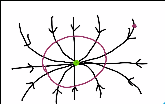
\includegraphics[scale=0.6]{orbits1.png}
        \end{center}
        \caption{}
        \label{fig:}
        \end{subfigure}
        \begin{subfigure}[b]{0.2\textwidth}
        \begin{center}
            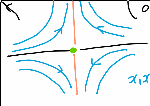
\includegraphics[scale=0.6]{orbits2.png}
        \end{center}
        \caption{}
        \label{fig:}
        \end{subfigure}
        \begin{subfigure}[b]{0.2\textwidth}
        \begin{center}
            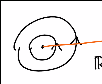
\includegraphics[scale=0.6]{orbits3.png}
        \end{center}
        \caption{}
        \label{fig:}
        \end{subfigure}
        \begin{subfigure}[b]{0.2\textwidth}
        \begin{center}
            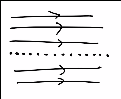
\includegraphics[scale=0.6]{orbits4.png}
        \end{center}
        \caption{}
        \label{fig:}
        \end{subfigure}
        \caption{Orbits in various cases.}%
        \label{fig:name}
    \end{figure}
    In the third case, the orbit space is $\R_{\geq 0}$. In the final case, even though the orbits are closed, the space is still not Hausdorff. In summary, $M/G$ may be non-Hausdorff in a very complicated way.
\end{exm}

Note that $M/G$ has a natural sheaf of functions. If $U \subset M/G$ is open, then $\pi^{-1}(U)$ is open in $M$, where $\pi: M \to M/G$ is the projection. We will declare the functions on $U$ to be the $G$-invariants. In the best case scenario, when $U$ is sufficiently small, we have $\pi^{-1}(U) = U \times G$ where the action is contained entirely in the second factor. Therefore functions on $U$ defined in the new sense are the same as normal functions on $U$.

However, there is no reason to expect this kind of behavior. We may get interesting behavior even for quotients by a finite group. For example, consider $M = \R^2$ and let $G = \{ \pm 1 \}$. Then $M / G$ is simply the closure of the upper half-plane with the negative and positive real axes glued together, so we obtain a cone with total angle $\pi$. We see that $\R^2 / \{ \pm 1 \}$ is a manifold near every point except $0$. At $0$, we study functions of the form $f(x_1,x_2)$ such that $f(-x_1,-x_2) = f(x_1,x_2)$, which are functions of $u = x_1^2, v = x_2^2, w = x_1x_2$. It is easy to see that these satisfy the equation $uv = w^2$.

Similarly, if we consider $\Z/m\Z$ acting on $\R^2$  by roots of unity, then we will obtain invariants $(u,v,w) = (x_1^m, x_2^m, x_1x_2)$ satisfying $uv = w^m$. This is known as the $A_{m-1}$ surface singularity.

\begin{rmk}
    Note that $\R^2 / \{ \pm 1 \}$ is very different from $\C / \{ \pm 1 \}$ because we take the second quotient in the category of complex manifolds. Here, $\C / \{ \pm 1 \} \simeq \C$ and the projection is a double cover branched at $0$. There is a similar result for $\C / \zeta_m$. 

    More generally, we have the following result: a finite subgroup $G \subset GL(n,\C)$ is generated by complex reflections if and only if $\C^n / G \simeq \C^n$. In general, $\C^n / (\text{finite subgroup of }GL(n,\C))$ is singular.
\end{rmk}

\begin{exm}
    Consider the permutation group $S_n \subset GL(n,\C)$. Each transposition $(ij)$ is a reflection in the hyperplane $x_i = x_j$. Therefore the coordinates on $\C^n / S_n$ are the elementary symmetric functions
    \[ e_k(x_1, \ldots, x_n) = \sum_{1 \leq i_1 < \cdots < i_k \leq n} x_{i_1} \cdots x_{i_k} \]
    for $k = 1, \ldots, n$. This is an important notion in representation theory because we can consider the map
    \[ GL(n, \F) / \text{conjugation} \xrightarrow{\text{eigenvalues}} \ol{\F}^n / S_n. \]
    In general, $S_n$ can be replaced by the Weyl group.
\end{exm}

In summary, $M/G$ may have complicated topology in singular. Complexity is good in math, but it is also good to have the simple cases. The best possible case is when the action is \textit{proper}, i.e. that the map $G \times M \to M \times M, (g,x) \mapsto (gx,x)$ is proper (ensures the quotient is Hausdorff), and \textit{free}, i.e. that there are no stabilizers.

\begin{thm}
    \label{thm:freeproper}
    Let $G \times M \to M$ be a free and proper action of a Lie group $G$ on a manifold $M$. Then $M/G$ is a manifold and the projection $M \xrightarrow{\pi} M/G$ is a locally trivial fibration with fiber $G$.
\end{thm}

\begin{exm}
    Here are some examples of a free and proper action:
    \begin{enumerate}
        \item The action of $G$ on $H \supset G$. Then $(g,h) \mapsto (gh,h)$ is an embedding and is in particular proper. Therefore $H/G$ is a manifold.
        \item Any free action of a compact Lie group.
    \end{enumerate}
\end{exm}


\begin{prop}
    The map $\pi: M \to M/G$ is open.
\end{prop}

\begin{proof}
    Note that $\pi^{-1}(\pi(V)) = \bigcup_{g \in G} g \cdot V$ is open.
\end{proof}

Note that the quotient by a group is a special case of a quotient by an equivalence relation.

\begin{prop}
    Suppose $\pi: M \to Y$ is open and a quotient by a closed equivalent relation. Then $Y$ is Hausdorff.
\end{prop}

\begin{proof}
    Suppose that $x,x'$ be such that $\pi(x,x') = (y,y')$ such that $(x,x') \notin R$. Then there exists a neighborhood of $(x,x')$ not intersecting $R$, so there exist $U,U' \ni x,x'$ such that $U \times U' \cap R = \emptyset$. These project to disjoint opens, so $Y$ is Hausdorff.
\end{proof}

In our situation, $R$ is the image of $G \times M \to M \times M$. By definition, the action is proper if this map is proper.

\begin{prop}
    Suppose $f: X \to Y$ is proper. Then the image of a closed set is closed.
\end{prop}

\begin{proof}
    It suffices to prove $f(X)$ is closed. Suppose $f(x_i) \to y_{\infty}$. Then $x_i \in f^{-1}(\{ f(x_i, y_{\infty}) \})$, which is compact. Thus we can find a subsequence $x_{k_i} \to x_{\infty} \in X$, so because $f$ is continuous, $f(x_{\infty}) = y_{\infty}$.
\end{proof}

In particular, in a Hausdorff space, all points are closed. In terms of our group action, this means all orbits are closed.

\begin{proof}[Proof of Theorem \ref{thm:freeproper}]
    Fix a point $x \in M$ and look at the neighborhood of $\pi(x)$. Consider the differential $\mf{g} \oplus T_x M \to T_x M$ of the action map $G \times M \to M$. Because this map has maximal rank everywhere, if we choose coordinates $\xi$ along $G.x$ and $\eta$ along $M$ and $\xi'$ for $G$, the differential is simply $(\xi',\xi,\eta) \mapsto (\xi'+\xi, \eta)$.

    Choose a submanifold $S$ transverse to the orbit, we can consider the action $G \times S \to M$. We see that this map is a local diffeomorphism, so we need $\pi^{-1}(\pi(S)) = G \times S$. This is not obvious and requires properness. One can imagine that there exists $g$ such that $gS \cap S \neq 0$ for any $S$. 

    Choose a sequence $S_n$ that shrinks to $x$. Then we consider the set $\{ g \mid g S_n \cap S_n \neq \emptyset \} \setminus \{1 \}$. Then we can consider
    \[ \qty{ g \mid g \ol{S}_n \cap \ol{S}_n \neq \emptyset } \]
    with a fixed neighborhood of $1$ removed. This is compact by properness. If $g$ lies in the intersection of all such sets, it must stabilize $x$, which is impossible.
\end{proof}

\begin{rmk}
    For algebraic actions, it is possible that $G.x$ is free but for all open $U$, $\mr{Stab}(x') \neq \{ e \}$ for all $x' \in U$. For an example, $SL(2,\C)$ acts on cubic polynomials in $x_1,x_2$. The generic polynomial has three roots and has stabilizer $\mu_3$, but $x_1^2 x_2$ has trivial stabilizer.
\end{rmk}

\begin{thm}
    Suppose the action of $G$ on $M$ is proper (but possibly not free). Then the normal bundle of $G.x$ is a vector space with an action of $G_x$, so there exists a neighborhood of $G.x$ isomorphic to $G \times N_x / G_x$. This is a vector bundle over the orbit with an action of $G$ (it is precisely the associated bundle).
\end{thm}

Now note that the stabilizer of $G_x$ is compact because the action is proper. We would like to find a $G_x$-invariant slice at $x$. To do this, we will need to discuss metrics. This is a smooth nondegenerate positive-definite quadratic form on each fiber. Then we can define the length of a curve by
\[ \int \sqrt{\norm{\dt{x}(t)}^2} \dd t. \]
There exist curves that minimize length locally, and these are called \textit{geodesics}. 

Then there is a map $T_x M \to M$ given by following a vector $v$ along the geodesic in the direction of $v$ for time $1$. This is a local diffeomorphism and is closely related to the exponential for Lie groups. Later in the lecture, we will prove that if $G$ acts on $M$ and $G$ is compact, then $M$ has a $G$-invariant Riemannian metric.

In particular, there is a $G_x$-invariant Riemannian metric on $M$. Then we can write $T_x M = T_x G \cdot x \oplus ( T_x G \cdot x )^{\perp}$. Identifying $(T_x G \cdot x)^{\perp}$ with the normal bundle $\nu_{ G \cdot x }$, then the slice is simply $S \coloneqq \exp(\nu_{G \cdot x})$.

Now consider the action $q: G \times S \to M$. If $h \in G_x$, then $q(gh,s) = q(g,hs)$ by definition. Therefore, we can write
\[ q: G \times S / G_x \to M, \]
where $G_x$ acts by $(g,x) \mapsto (gh^{-1},hs)$. This is $G$-equivariant and locally an isomorphism.

\begin{thm}
    This is an isomorphism of $G \times N_x / G_x \to M$ is a neighborhood of the orbit of $x$. Note that we can scale any $\R^n$ to the unit ball.
\end{thm}

\begin{cor}
    The neighborhood of the orbit of $x$ in $M / G$ looks like $N_x / G_x$.
\end{cor}

\begin{cor}
    The stabilizer of any nearby point is conjugate to a subgroup of $G_x$.
\end{cor}

\begin{rmk}
    Sometimes the quotient $G \times Y / H$ by the action $(g,y) \mapsto (gh^{-1},hy)$ is denoted by $G \times_H Y$.
\end{rmk}

\begin{cor}
    The manifold $M$ has a $G$-invariant metric.
\end{cor}

\begin{proof}
    Let $h \in G_x$. Then for a vector $v \in T_{gx}M$, we can associate $g^{-1}v$ and $h^{-1} g^{-1}v$ to $v$, but these must have the same length because they differ by an element of the stabilizer. This gives an invariant metric in a neighborhood of the orbit. Finally, we can sum the local metrics over a partition of unity to obtain a global invariant metric.
\end{proof}

\begin{thm}
    Let $H$ be a compact Lie group acting on a manifold $M$. Then $M$ has an $H$-invariant metric.
\end{thm}

\begin{proof}
    Choose some Riemannian metric $\norm{-}_0$ on $M$. Then choose a Haar measure on $H$ and define
    \[ \norm{v}^2 \coloneqq \int_H \dd h \norm{h \cdot v}_0^2. \]
    To show invariance, note that
    \[ \norm{g \cdot v}^2 = \int_H \dd h \norm{g \cdot h \cdot v}_0^2 = \int_H \dd(g^{-1}h') \norm{h' \cdot v}_0^2 = \int_H \dd h' \norm{h' \cdot v}_0^2. \qedhere \]
\end{proof}

More generally, suppose $H$ acts on an affine linear space by affine transforations and suppose there is a closed convex $H$-invariant subset $B$. Then there exists an $H$-fixed point (by the same integration argument).

Now we will show existence of the Haar measure. Recall that $T H \simeq T_1 H \times H$ by left translation. Then we may choose an $\mf{h}$-valued $1$-form $g^{-1} \dd g$ on $H$, and this gives a finite volume form if the group is compact.

\chapter{Classification of Lie Groups}%
\label{cha:classification_of_lie_groups}

\section{Topology of Lie Groups}%
\label{sec:topology_of_lie_groups}

Recall that if $G$ acts on $M$ properly and freely then $\pi: M \to M/G$ is a locally trivial fibration with fiber $G$ and $M/G$ is a manifold. Now suppose $H$ is a Lie subgroup of $G$. Then $H$ acts freely and properly on $G$. Therefore we have a map $G \to G/H$ and $G/H$ is a manifold. Our goal is to use this fibration to understand the geometry of its ingredients.

\begin{exm}
    Consider $G = SU(2) \simeq S^3$ and let $H$ be the set of diagonal matrices in $G$. Then to compute $G/H$, note that $G$ acts on $\C^2$ and hence on $\C\P^1$. The stabilizer of a point is $H$, and thus $G \to G/H$ is the \textit{Hopf fibration} $S^1 \to S^3 \to S^2$. An illustration of the Hopf fibration is below:
    \begin{figure}[H]
        \centering
        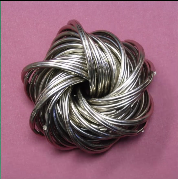
\includegraphics[scale=1]{hopf}
        \caption{The Hopf fibration}%
        \label{fig:hopf}
    \end{figure}
    Any two fibers are linked as the Hopf link, so this is not a globally trivial fibration.
\end{exm}

\begin{exm}
    Consider $G = SU(2)$ acting on itself by conjugation. This fixes $1 \in G$, so it acts by conjugation on $\mf{g} = T_1 G = \{ \xi \in M_2(\C) \mid \xi + \xi^{\dag} = 0, \trace \xi = 0 \}$. Because the norm of the matrix is preserved, we have a map $SU(2) \to SO(3, \R)$ with kernel the center of $SU(2)$, which is just $\{ \pm 1 \}$. By dimension arguments, the map is surjective, and thus we have realized $SO(3, \R) \simeq \R \P^3$.
\end{exm}

We can discuss various topological invariants of Lie groups, in particular their homotopy, homology, and cohomology groups. We will begin with $\pi_0(X)$, the set of connected components. If $G$ is a Lie group, then $\pi_0(G)$ is a \textbf{group} isomorphic to $G / G_0$, where $G_0$ is the connected component of the identity. It is clear that $\pi_0(G/H) = \pi_0(G) / \Im \pi_0(H)$ under the natural map $\pi_0(H) \to \pi_0(G)$.

\begin{exm}
    Let $G = SU(2)$ and let $H = Z(SU(2))$. Then any path connecting $\pm 1$ in $G$ descends to $G/H \simeq \R\P^3$, so the kernel of $\pi_0(H) \to \pi_0(G)$ is exactly the image of the transport $\pi_1(G/H) \to \pi_0(H)$.
\end{exm}

Recall that we have a long exact sequence
\[ \cdots \to \pi_1(H) \to \pi_1(G) \to \pi_1(G/H) \to \pi_0(H) \to \pi_0(G) \to \pi_0(G/H) \to 1 \]
arising from the fibration. 

\begin{thm}
    Let $G$ be a topological group. Then $\pi_1(G)$ is abelian.
\end{thm}

\begin{proof}
    The homotopy $[0,1] \times [0,1] \to G, (t,s) \mapsto \gamma_1(t) \gamma_2(s)$ exhibits a homotopy between $\gamma_1 \gamma_2$ and $\gamma_2 \gamma_1$ for two loops $\gamma_1, \gamma_2$ based at the identity.
\end{proof}

\begin{rmk}
    $\pi_1(\R^2 \setminus \pm 1)$ is not abelian. In fact it is equal to $\Z * \Z = F_2$.
\end{rmk}

Let $\wt{X} \xrightarrow{\pi} X$ be a covering space. Then we have a map $\pi_1(X) \to \wt{x} \to X$ given by transport, and if $\pi_1(\wt{X}) = 1$, then $\wt{X}$ is the universal cover.

\begin{prop}
    If $G$ is a Lie group then so is its universal cover $\wt{G}$ by multiplication $\gamma_1(t) \gamma_2(t)$.
\end{prop}

\begin{cor}
    If $G$ is a connected Lie group, then there exists a unique simply connected Lie group $\wt{G}$ such that $1 \to \pi_1(G) \to \wt{G} \to G \to 1$ is an exact sequence.
\end{cor}

\begin{exm}
    The map $SU(2) \to SO(3, \R)$ is a universal covering. An even more basic example is the cover $0 \to \Z \to \R \to S^1 \to 1$.
\end{exm}

\begin{prop}
    Suppose $G$ is a connected Lie group and $\Gamma \subset G$ is a discrete normal subgroup. Then $\Gamma \subset Z(G)$.
\end{prop}

\begin{proof}
    Let $\gamma \in \Gamma$ and consider the map $G \ni g \mapsto g \gamma g^{-1} \in \Gamma$. Because $G$ is connected, the image is a point, which must be $\gamma$ because we can choose $g = 1$.
\end{proof}

In summary, any connected Lie group $G$ has the form $\wt{G} / \Gamma$, where $\wt{G}$ is simply connected and $\Gamma$ is a discrete subgroup of the center.

\begin{cor}
    If $G$ is abelian, then $G$ is of the form $\R^n / \Lambda$, where $\Lambda$ is some discrete subgroup, and this means that $G \simeq \R^k \times (S^1)^{n-k}$.
\end{cor}

\begin{rmk}
    This allows us to prove the fundamental theorem of algebra. If $\F/\R$ is a field extension, then $( \F^* )_0$ is abelian and connected. Then for $d = 1$, this is $\R$, for $d = 2$ this is $S^1 \times \R$, and for $d \geq 3$ this is $S^{d-1} \times \R$, which is impossible.
\end{rmk}


Here is a very important ideal in Lie theory: Consider a Lie group $G$ with identity $1$. Then if we consider $\mf{g} = T_1 G$, we can reconstruct a lot of information about $G$. An obvious limitation of this approach is that some Lie groups are locally isomorphic.

\begin{exm}
    Recall that $SU(2)$ is a double cover of $SO(3)$, so they are locally isomorphic. In particular, any group $G$ is locally isomorphic to $G / \Gamma$, where $\Gamma \subset Z(G)$ is discrete.
\end{exm}

Our strategy for dealing with this is to determine the universal cover, which is equivalent to determining $\pi_1(G)$. We will see later that simply-connected Lie groups are determined by the infinitesimal data.

Previously, we discussed the long exact sequence arising from a fibration. To make this precise, we need to define $\pi_n(X,*)$. But this is simply the group $[S^n, X]^0$ of homotopy classes of based maps from $S^0$ to $X$. For $n > 1$, we can see that $\pi_n$ is commutative by the following picture (or the fact that $S^n$ is a double suspension).
\begin{figure}[H]
    \centering
    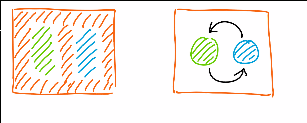
\includegraphics[width=0.8\linewidth]{pinab}
    \caption{Proof that $\pi_2$ is abelian by picture}%
    \label{fig:pinab}
\end{figure}

Very often, $G/H$ is a sphere, with homotopy groups
\[ \pi_k(S^n) = \begin{cases}
    0 & k < n \\
    \Z & k = n \\
    ??? & k \gg n
\end{cases}. \]
Not much is known about the higher homotopy groups of spheres, and computing them is a central problem in modern algebraic topology. Fortunately, it is easier to compute the homotopy groups of Lie groups.

\section{Lie Algebras}%
\label{sec:lie_algebras}

We will discuss reconstruction of simply-connected Lie groups from their local data. This can be phrased as an equivalence of categories. On one side, we have the category of simply-connected Lie groups, and on the other side, we have the category of Lie algebras. We will define a functor $\operatorname{Lie}$ from Lie groups to Lie algebras that is an equivalence of categories.

We will define $\Lie(G) = T_1(G)$ plus some extra data, and for any $f \colon G \to G'$, we wil define $\Lie(f) = \dd f \colon T_1 G \to T_1 G'$.

\begin{exm}
    Let $f \colon \R \to \R$ be a Lie group homomorphism. Then we can differentiate to see that 
    \[ \eval{\dv{y}}_{y = 0} f(x+y) = f'(x) = f'(0). \]
    This means that the morphism is determined by an ODE, and so it must be linear. Then $f'(0)$ is precisely the map between Lie algebras.
\end{exm}

In general for $f \colon G \to G'$, then we can differentiate with respect to $g_2$ at $g_2 = 1$ to obtain a system of first order ODEs. Then solvability of these ODEs is a condition on $\dd f$ that is equivalent to being a homomorphism of Lie algebras.

\begin{defn}
    A Lie algebra is a vector space $\mf{g}$ with a bilinear operation
    \[ [-,-] \colon \mf{g} \otimes \mf{g} \to \mf{g} \]
    such that $[x,x] = 0$ that satisfies the Jacobi identity:
    \[ [z, [x,y]] + [y, [z,x]] + [x, [y,z]] = 0. \]
\end{defn}

We will construct the Lie bracket out of multiplication in $G$. If we simply differentiate the multiplication $m$, the differential 
\[ \dd m \colon T_1 G \oplus T_1 G \to T_1 G \]
is simply the addition. This is a linear map, but it tells us that all Lie groups are the same locally.

Therefore, we need to consider higher order terms in the Taylor expansion of $m$. This is
\[ m(\xi, \eta) = 0 + (\xi + \eta) + \text{quadratic terms} + \cdots \]
and the quadratic term is a bilinear form $B(\xi, \eta)$ with no quadratic terms in $\xi$ or $\eta$. This is \textbf{not} independent of the coordinates because if we choose $\xi' = \xi + Q(\xi), \eta' = \eta + Q(\eta)$, then the multiplication becomes
\[ m(\xi', \eta') = \xi + \eta + B(\xi, \eta) + Q(\xi + \eta) + \cdots \]
In barticular, we have $B' = B + Q(\xi + \eta) - Q(\xi) - Q(\eta)$, which does not necessarily vanish. However, it is symmetric, so we can define the \textit{Lie bracket} 
\[ [\xi, \eta] = B(\xi, \eta) - B(\eta, \xi). \]

\begin{quotation}
    \itshape In mathematics, there is a high road and a low road. The low road is to write everything in coordinates, which is sort of what we did here. It's good to be able to take the low road, for example when we need to compute with a computer. \sourceatright{A. Okounkov}
\end{quotation}

\begin{rmk}
    There are many other definitions of the Lie bracket. 
    \begin{enumerate}
        \item We can consider the commutator in $G$. If we assume $G \subset GL(n, \F)$, then we have $[\xi, \eta] = \xi \eta - \eta \xi$. The differential of the commutator vanishes, but the second differential is precisely the bracket.
    \end{enumerate}
\end{rmk}

We need to prove that the commutator satisfies the Jacobi identity, which can be restated as
\[ [x, [y,z]] = [[x,y],z] + [y, [x,z]]. \]
Now define $\mr{ad}_x(-) = [x,-]$. Then the Jacobi identity says that $\mr{ad}_x$ is a derivation of the Lie bracket.

Note that if $V$ is a vector space with $\star \colon V \otimes V \to V$, then $\Aut(\star) \subset GL(V)$ is an algebraic subgroup. If we apply the Lie functor, we see that
\[ \Lie ( \Aut(\star) ) = \qty{ D \in \mf{gl}(V) \mid D(y \star z) = D(y) \star z + y \star D(z) }. \]
Consider the adjoint action of $G$ on itself. This fixes $h = 1$, so it gives a representation of $G$ on $\mf{g} = T_1 G$. If $G$ is a matrix group, then this is really a product $\xi \mapsto g \xi g^{-1}$. If we write this out in coordinates, we see that the adjoint representation $\mr{Ad}$ of $G$ takes values in $\Aut([-,-])$ and thus when we differentiate. If we take the derivative $\mr{ad} = \dd_1 \mr{Ad}$, we obtain a map
\[ g \to \Der([-,-]) \subset \mf{gl}(\mf{g}). \]
We simply need to check that $\mr{ad}_x = [x,-]$. But this is obvious because the left hand side comes from differentiating $ghg^{-1}$ and the right hand side comes from differentiating $ghg^{-1}h^{-1}$.

\begin{rmk}
    This gives yet another definition of the Lie bracket.
\end{rmk}

\section{Correspondence between Lie groups and Lie algebras}%
\label{sec:correspondence_between_lie_groups_and_lie_algebras}

Now let $M$ be a smooth manifold with an action of a Lie group $G$. Then $C^{\infty}(M)$ is an algebra that is acted on by $G$. Then we know that $\Der(C^{\infty}(M))$ is simply the space of vector fields. Then we can write $f(x) = f(x_0) + \dd f + \mf{m}_x^2$, where $\mf{m}_x$ is the ideal of functions that vanish at $x_0$. For any derivation, $\eval{ D(\mf{m}_x^2)  }_{x = x_0} = 0$. This defines a tangeng vector at any $x_0 \in M$. In particular, $\mf{g}$ defines $C^{\infty}$ vector fields on $M$. Then we know that derivations form a Lie algebra.

For example, consider the action of $G$ on itself by left translation. Then we have a map $\mf{g} \to H^0(G, TG)$. In addition, it is easy to see that this gives right-invariant vector fields on $G$. On the other hand, right-invariant vector fields are determined by their value at $1$, so we have an isomorphism $H^0(G, TG)^G \simeq \mf{g}$ of vector spaces. In fact, this can be upgraded to an isomorphism of Lie algebras.

Returning to the main point, we want to prove
\begin{thm}
    The functor $\Lie \colon \qty{ 1\text{-connected Lie groups} } \to \qty{\text{Lie algebras}}$ is an equivalence of categories.
\end{thm}

\begin{thm}
    Let $G_1, G_2$ be connected Lie groups with $\Lie(G_i) = \mf{g}_i$. Then any homomorphism $f \colon G_1 \to G_2$ is uniquely determined by $\dd f \colon \mf{g}_1 \to \mf{g}_2$. 
\end{thm}

\begin{proof}
    We know that $f(g_1 g_2) = f(g_1) f(g_2)$. Then if we differentiate with respect to $g_1 = 1 + \xi$, then
    \[ \dv{\xi} f(g) = f(\xi) \cdot f(g). \]
    This gives us a system of first order ODE. By connectedness, there is a unique solution with prescribed initial condition.
\end{proof}

Later, we will see that the mixed partials are equal (or the curvature vanishes) if and only if $\dd f$ is a Lie algebra homomorphism.

\begin{rmk}
    There is no homomorphism of Lie groups from $G_1 \colon \R / \Z \to \R = G_2$ corresponding to the identity homomorphism between the Lie algebras.
\end{rmk}

These ODE that we obtain from differentiating the multiplication naturally lead to the concepts of connections and curvature. Suppose we have a locally trivial fiber bundle over a base $B$ with fibers $F$. Then the idea of a connection is to be able to lift paths downstairs to paths upstairs respecting concatenations of paths.

Fix a Lie group $G$ acting on the fiber $F$. Then we say the \textit{structure group} is contained in $G$ if all transition functions may be chosed to be in $G$. For example, a vector bundle is a locally trivial bundle with structure group $GL(n)$. We can use the same transition functions to glue copies of $G$, and we obtain a principal bundle $\mc{P}$. Then the old bundle can be obtained using the associated bundle construction $\mf{P} \times_G F$ and a connection on a principal $G$-bundle induces a connection on any associated bundle.

In our case, we are talking about the trivial $G$-bundle over $H$. Then sections are maps from $H$ to $G$. In coordinates, these are lifts that are invariant under the action of $G$ on the right. This means we can consider the value at $1 \in G$, which means we have a map $ \alpha \colon T_b B \to \mf{g}$. Thus a connection can be thought of as a right-invariant Lie algebra-valued $1$-form. However, this is dependent on the trivialization. If we change the section by a function $g(b)$, we know a section is contant if 
\[ \dv{\xi} - \alpha(\xi) = 0. \]
However, if we conjugate by $g$, then we need to differentiate $\dd (g^{-1}) = - g^{-1} \dd{g} g^{-1}$, and obtain
\[ \dv{\xi} - \wt{\alpha}(\xi) = 0, \]
where $\wt{\alpha} = g \alpha g^{-1} + \dd{g} \cdot g^{-1}$.

Next, when does the transport along the path depend only on the endpoints? We can consider
\begin{enumerate}
    \item Small changes, i.e. homotopies with fixed endpoints. In this case, the connection is \textit{flat}.
    \item Paths up to homotopy, i.e. $\pi_1(B)$.
\end{enumerate}

\begin{prop}
    A connection is flat if and only if its curvature is identically zero.
\end{prop}

The curvature is a certain $2$-form that measures the difference between two solutions to an ODE. If we transport along $\xi_1 \xi_2 \xi_1^{-1} \xi_2^{-1}$, then we obtain the commutator
\[ \qty[ \pdv{\xi_2} - \alpha_2, \pdv{\xi_1} - \alpha_1 ] = - \qty( \pdv{\xi_2} \alpha_1 - \pdv{\xi_1} \alpha_2 + [\alpha_2, \alpha_1] ). \]
Thus if the connection is flat, then the curvature vanishes. In the other direction, suppose we have two homotopic paths. Then if we break down the square $[0,1]^2$ into squares of size $\ep$, then each square changes the result by $\ep^2 \cdot \text{curvature} + O(\ep^3)$, and so if we make $\ep$ small enough, the change vanishes.

Returning to our original problem, suppose we have a map $f \colon H \to G$. Then $\dd{f} \colon \mf{h} \to \mf{g}$ determines a connection on $G \times_H H$. On $H$ we have the canonical $1$-form $\dd{h} \cdot h^{-1}$ If $\dd{f}$ is a Lie algebra homomorphism, then 
\[ [\dd{f}(\xi_1), \dd{f}(\xi_2)] = \dd{f} ( [\xi_1, \xi_2] ) \]
and thus the curvature of the connection $\alpha$ induced from $\dd{h} \cdot h^{-1}$ is the differential of the curvature of $\dd{h} \cdot h^{-1}$, which is identically zero.

\begin{rmk}
    All of this can be expressed in elementary terms. First, we have $\pdv{\xi_i} g = \alpha_i g$. Then we have
    \[ 0 = \pdv{g}{\xi_i}{\xi_j} - \pdv{g}{\xi_j}{\xi_i} = \qty( \pdv{\alpha_j}{\xi_i} - \pdv{\alpha_i}{\xi_j} + [\alpha_i, \alpha_j] ) g. \]
    Thus we have proved the following theorem:
\end{rmk}

\begin{thm}
    If $H$ is a simply connected Lie group and $\varphi \colon \Lie H \to \Lie G$ is a Lie algebra homomorphism, then there a unique map $f \colon H \to G$ such that $\eval{\dd{f}}_1 = \varphi$.
\end{thm}

For example, if we want to prove that $\log(xy) = \log x + \log y$, we write
\[ \log(xy) = \int_1^x \frac{\dd{t}}{t} + \int_x^{xy} \frac{\dd{t}}{t} \]
and note that the second term in the sum equals $\int_1^y \frac{\dd{t}}{t}$.

Recall the differential equations that we constructed for a homomorphism of Lie groups from the Lie algebra. These equations are right-invariant in both the source and the target and imply that $f$ is a homomorphism.

\begin{exm}
    Here is a silly example: Note the isomorphism $(\R_{>0}, \times) \to (\R, +)$. Then $f(xy) = f(x) + f(y)$ and so we have
    \[ y \dv{y} f = c \]
    for some constant $c$. In the other direction, we have $\varphi(x+y) = \varphi(x) \varphi(y)$, so 
    \[ \dv{y} \varphi = c \cdot \varphi \]
    for some constant $c$. The solution to the second equation is clearly the exponential function, and the solution to the first is
    \[ f(y) = \int_1^y c \frac{\dd{t}}{t} \eqqcolon c \log y. \]
    Invariance implies that $\log$ is a homomorphism.
\end{exm}

\begin{thm}[Lie]
    For any simply connected Lie group $G$, the map
    \[ \Hom_{\text{Lie Groups}}(H,G) \xrightarrow{\dd} \Hom_{\text{Lie Algebras}}(\Lie(H), \Lie(G)) \]
    is an isomorphism.
\end{thm}

Here are some applications:
\begin{enumerate}
    \item Any connected abelian Lie group $G$ of dimension $n$ is of the form $\R^n / \Gamma$, where $\Gamma \cong \Z^k$. Thus $G = (S^1)^k \times \R^{n-k}$.
    \item Not all Lie groups are matrix Lie groups. However, every Lie algebra is a matrix Lie algebra in characteristic $0$. In the category of Lie algebras, we can always lift the adjoint representation $\ad \colon \mf{g} \to \mf{gl}(\mf{g})$ to the center of $\mf{g}$. However, when we consider the adjoint representation of $G$ as a Lie group, we cannot lift to the center.

        For example, consider $SL(2, \R)$. This has $\pi_1(SL(2, \R)) = \Z$. Then $G = \wt{SL(2, \R)}$ has $\Z$ in the center, and so any map
        \[ f \colon G \to GL(N, \C) \]
        corresponds to a map of Lie algebras $\mf{sl}(2, \R) \to \mf{gl}(N, \C)$. This gives a map $\mf{sl}(2, \C) \to \mf{gl}(N, \C)$, which then lifts to a map $SL(2, \C) \to GL(N, \C)$. In particular, all linear representations of $G$ factor through $SL(2, \C)$ are are thus trivial on the center.
\end{enumerate}

\begin{defn}
    Suppose $G$ is a real Lie group with Lie algebra $\mf{g}$. Then if we take the complexification $\mf{g} \otimes_{\R} \C$, this gives a map $G \to G_{\C}$ for $G_{\C}$ the complex Lie group corresponding to $\mf{g}_{\C}$. We say that $G_{\C}$ is a \textit{complexification} of $G$ and that $G$ is a \textit{real form} of $G_{\C}$.  
\end{defn}

\begin{rmk}
    Note that this relation is generally many-to-one. In particular, both $SL(n, \R)$ and $SU(n)$ are real forms of $SL(n, \C)$.
\end{rmk}

Now let $G$ be a Lie group and $\xi \in \mf{g}$. Then $\R \ni t \mapsto t \xi \in \mf{g}$ is a homomorphism of Lie algebras. Thus there exists a unique map
\[ \R \ni t \mapsto \exp(t \xi) \in G \]
and this is the matrix exponential for matrix groups. Also, $\dv{t} \exp(t \xi) = \xi \exp(t \xi)$. In addition, if $[\xi, \eta] = 0$, then we can exponentiate $\exp(t \xi + s \eta) = \exp(t \xi) \exp(s \eta)$ in either order.

\begin{thm}[Lie]
    For any Lie algebra $\mf{g}$ over $\R$ or $\C$, there exists a unique simply-connected Lie group $G$ with Lie algebra $\mf{g}$.
\end{thm}

This gives a correspondence between our linear local data and nonlinear global data. We can construct manifolds either as:
\begin{enumerate}
    \item A quotient of something simpler. If $G$ is a simply-connected Lie group, then if we choose a point $x \in \mf{g}$, then we can consider smooth paths $g$ from $1$ to $x$. Then $\dt{g}(t) g^{-1}(t) = \xi(t)$ the tangent vector at time $t$, and for a smooth homotopy between paths, If the curvature vanishes, then we have
        \[ \pdv{s} \xi - \pdv{t} \eta = [\xi, \eta]. \]
        Then we can write $G$ as the paths in the Lie algebra modulo solutions to the equation. Fortunately, the analysis reduces to first-order deformations.
    \item As a ``submanifold'' of something simpler. Write $\mf{g} \hookrightarrow \mf{gl}(n, \R)$. Then we have a map $G \to GL(n, \R)$ with some kernel $\Gamma$. Thus $G$ is the universal cover of $G/\Gamma \subset GL(n, \R)$. Therefore, at least locally, every element of the Lie group is a matrix.

        A problem with this approach is that $G/\Gamma$ need not be a submanifold. If we have the map $\R \to \R^2 / \Z^2$ with dense image, we obtain a foliation, so individual leaves are (locally) submanifolds, but we do not globally obtain a submanifold. In particular, if $H \to G$ is an injective Lie algebra homomorphism, we have a foliation with leaves corresponding to the cosets of $H$ in $G$.
\end{enumerate}


\end{document}
